\documentclass[11pt,a4paper,twoside]{book}
% add draft to the options to make the compile go faster

%\synctex=1

%packages
\usepackage{varioref} % cool references to pages etc
\usepackage{hyperref} % make links

\usepackage{url}						% urls (duh)
\usepackage{doi}						% doi links
\usepackage{a4wide}						% iets meer tekst op 1 pagina
\usepackage[dutch,english]{babel}	  	% nederlands en engels inladen
\usepackage{amsmath}					% AMS-wiskundige symbolen
\usepackage{amssymb} 					% invoegen van reele getallen etc
\usepackage[]{graphicx}					% figuren invoegen
% if you want to speed up things:
% \usepackage[draft]{graphicx}					% figuren invoegen
\usepackage{float}						% positie figuren etc.
\usepackage{subfloat}						% positie figuren etc.
\usepackage[hang,bf]{caption}	        % captions van figuren: vet en goed gealigneerd
\usepackage{subcaption}						% positie figuren etc.
\usepackage{pdfpages}					% pdf pagina's invoegen

\usepackage[toc]{glossaries}            % list of abbriviations
\usepackage{imakeidx}                           % list of abbriviations - not used

\usepackage{rotating}                   % tables, figures, ... rotated 
\usepackage{arydshln}                   % advanced package for tables: dashed lines etc
\usepackage[shortcuts]{extdash}         % more types of dashes, sometimes useful
\usepackage{booktabs} % Allows the use of \toprule, \midrule and \bottomrule in tables for horizontal lines
\usepackage{cancel}						% cancelen van termen in wiskundige uitdrukkingen

\usepackage{emptypage}                  % allows inclusion of empty pdf pages

\usepackage[utf8]{inputenc} % use UTF-8, to make life easier

\usepackage[square,numbers,sort&compress]{natbib}
\usepackage{nicefrac}
%\usepackage{subfig} % outdated

%\usepackage{algorithm} % nice environment for pseudocode
%\usepackage{algpseudocode} % pseudocode

\usepackage{bookmark}
\usepackage{mathrsfs}
\usepackage{xcolor} % kleurtjes
\usepackage{listings} % om source code netjes weer te geven
\usepackage[nottoc]{tocbibind} % Bibliografie in ToC; maar de ToC zelfs niet in de ToC

\usepackage{braket} % bra ket stuff
\usepackage{csquotes} % nice quotes
\usepackage{amsthm} % for \newtheorem commands
\usepackage[toc,page]{appendix}
\usepackage{mathtools} % for dcases
\usepackage{bbold} 
\usepackage{dsfont} 
\usepackage{chemfig} 
\usepackage{combelow} % Typeset "comma-below" letters, as in Romanian
\usepackage{memhfixc} % for \cleartorecto and \cleartoverso

\usepackage{afterpage} 
% create new blank pages with no style until the next uneven page, not do always work?
\newcommand\blankpage{%
    \null
    \thispagestyle{empty}%
    \addtocounter{page}{-1}%
    \newpage}

\usepackage{epigraph} % for nice quotes in chapters

\usepackage{bibentry} % for list of publications in appendix

% indenting multiline footnotes
\usepackage{scrextend}
\deffootnote{0em}{1.6em}{\thefootnotemark.\enskip}

\usepackage{etoolbox}
% bordermatrix with [ ] instead of ( )
\let\bbordermatrix\bordermatrix
\patchcmd{\bbordermatrix}{8.75}{4.75}{}{}
\patchcmd{\bbordermatrix}{\left(}{\left[}{}{}
\patchcmd{\bbordermatrix}{\right)}{\right]}{}{}

% less white space before subequation
\preto\subequations{\ifhmode\unskip\fi}

% packages not used, but perhaps interesting
%\usepackage{pifont}
%\usepackage{ulem}
%\usepackage{soul}
%\usepackage{makeidx}                    % index
%\usepackage{slantsc}
%\usepackage{placeins}
%\renewcommand*\sfdefault{uop}
%\renewcommand*\familydefault{\sfdefault} 


%% hypersetup
\hypersetup{
    pdfauthor={Aranka Steyaert},
    pdftitle={TBD},
    pdfkeywords={tbd},
    pdfsubject={},
%    plainpages=false,
    pdfcreator={\LaTeX\ with package \flqq hyperref\frqq}
    pdfpagelabels,
    bookmarksopen=true,
    bookmarksnumbered=true,
    unicode=true,
}		

\newcommand{\minus}{\scalebox{0.75}[1.0]{$-$}} % short minus sign

% papersize required for FEA
\usepackage{geometry}
\geometry{papersize={16cm,24cm},layoutsize={16cm,24cm},top=2cm,bottom=2cm,left=2cm,right=2cm}
\usepackage[strict]{changepage}

% font
\usepackage[T1]{fontenc}
%\usepackage{bera}
\usepackage{libertine}
\renewcommand*\familydefault{\sfdefault}  % biolinum
%\usepackage{libgreek}
%\usepackage[libertine]{newtxmath}

\usepackage{eucal}
%\usepackage{kpfonts}					% ander lettertype
%\usepackage[sc]{mathpazo}
%\linespread{1.05}         % Palatino needs more leading (space between lines)
%\usepackage[T1]{fontenc}

%\usepackage{lmodern} % load a font with all the characters
%\renewcommand*\familydefault{\sfdefault}  % biolinum

%header
\usepackage{fancyhdr}
\pagestyle{fancy}
\widowpenalty=1000
\clubpenalty=1000
\hyphenpenalty=500

\fancyhead[RE]{\slshape \rightmark}
\fancyhead[LO]{\slshape \leftmark}
\fancyhead[RO]{}
\fancyhead[LE]{}

% alinea
\setlength{\parindent}{0pt}
\setlength{\parskip}{1ex plus 0.5ex minus 0.2ex}

\AtBeginEnvironment{adjustwidth}{\partopsep0pt}

% subsubsection: different type of numbering (not 1.11.2 but just roman numbers)
\setcounter{secnumdepth}{3} 	                % nummers tot op diepte 3
\def\thesubsubsection{\Roman{subsubsection}.}	% Romeinse cijfers als index voor subsubfigure

% title of chapter
\renewcommand{\chaptermark}[1]{
\markboth{#1}{}
}

% tocdept in table of content
\renewcommand{\sectionmark}[1]{\markright{#1}}
\setcounter{tocdepth}{1}

\setcounter{tocdepth}{3}
\setcounter{secnumdepth}{3}

%nieuwe commandos
\newcommand{\pafgeleide}[2]{\frac{\partial #1}{\partial #2}}			% partiele afgeleide
\newcommand{\ptweeafgeleide}[3]{\frac{\partial^2 #1}{\partial #2 \partial #3}}
\newcommand{\afgeleide}[2]{\frac{\mathrm{d} #1}{\mathrm{d} #2}}			% afgeleide
\newcommand{\subsafgeleide}[2]{\frac{\mathrm{D} #1}{\mathrm{D} #2}}		% substantiele afgeleide
\newcommand{\diff}{\mathrm{d}}						 	% rechte d voor dx bvb
\newcommand{\ltransf}{\stackrel{\mathcal{L}}{\longleftrightarrow}}		% pijl laplace
\newcommand{\laplace}{\mathcal{L}}						% teken laplace
\newcommand{\heaviside}{\mathbb{H}}						% Heavisidefunctie
\newcommand{\abs}[1]{\left|#1\right|}						% absolute waarde
\newcommand{\gehelegetallen}{\mathbb{Z}}					% symbool gehele getallen
\newcommand{\complexegetallen}{\mathbb{C}}					% symbool complexe getallen
\newcommand{\verz}[1]{\left\{ #1 \right\}}					% accolades
\newcommand{\vnabla}{\vec{\nabla}}						% Nabla met een vectorteken erboven
\newcommand{\tens}[1]{\boldsymbol{#1}}						% tensorteken
\renewcommand{\vec}[1]{\boldsymbol{#1}}						% vectorteken
\newcommand{\odd}{\mathcal{O}}							% oneven
\newcommand{\even}{\mathcal{E}}							% even
\newcommand{\vet}[1]{\boldsymbol{#1}}						% iets in het vet plaatsen in math omgeving		

\newcommand{\tr}[1]{\mathrm{Tr}\left(#1\right)}
\newcommand{\erdm}[1]{\rho_{#1}}
\newcommand{\trdm}[1]{\Gamma_{#1}}
\newcommand{\drdm}[1]{{^3 \Gamma_{#1}}}

\newcommand{\padd}[1]{\hat{a}_{#1}^{\dagger}}
\newcommand{\pdel}[1]{\hat{a}_{#1}}

\newcommand{\citew}[1]{\citeauthor{#1} \citep{#1}}

\newcommand{\todo}[1]{{\color{red}{\textbf{Todo: #1}}}}
% to hide the todos, replace line above with:
%\newcommand{\todo}[1]{}

\newcommand{\dth}{$\text{D}_\text{2h}$}
\newcommand{\co}{$\text{C}_\text{1}$}
\newcommand{\ctv}{$\text{C}_\text{2v}$}

\newcommand\norm[1]{\left\lVert#1\right\rVert}


%physical properties
\newcommand{\efield}{\mathcal{E}}														% even

% Clebsch-coefficienten
\newcommand{\cgc}[6]{ \left\langle #1 \: #2 \; #3 \: #4 \right| #5 \: #6 \left.\right\rangle }

% 3j symbolen
\newcommand{\driej}[6]{
    \left(
    \begin{array}{ccc}
        #1 & #3 & #5 \\
        #2 & #4 & #6
    \end{array}
    \right)
}

% reduced matrix element
\newcommand{\rme}[3]{\bigl\langle #1 \bigl|\bigl| #2 \bigr|\bigr| #3 \bigr\rangle}		

\makeatletter
\newcommand{\pushright}[1]{\ifmeasuring@#1\else\omit\hfill$\displaystyle#1$\fi\ignorespaces}
\newcommand{\pushleft}[1]{\ifmeasuring@#1\else\omit$\displaystyle#1$\hfill\fi\ignorespaces}
\newcommand{\specialcell}[1]{\ifmeasuring@#1\else\omit$\displaystyle#1$\ignorespaces\fi}
\makeatother

\graphicspath{{figures/}}

\hyphenation{re-pre-sen-ta-bil-it-y}

\newacronym{a}{A}{Adenine}
\newacronym{bp}{bp}{base-pairs}
\newacronym{c}{C}{Cytosine}
\newacronym{crf}{CRF}{Conditional Random Field}
\newacronym{dna}{DNA}{Deoxyribonucleic Acid}
\newacronym{g}{G}{Guanine}
\newacronym{ngs}{NGS}{Next-Generation Sequencing}
\newacronym{pgm}{PGM}{Probabilistic Graphical Model}
\newacronym{rna}{RNA}{Ribonucleic Acid}
\newacronym{sms}{SMS}{Single Molecule Sequencing}
\newacronym{t}{T}{Thymine}
\newacronym{sbs}{SBS}{Sequencing by Synthesis}

\newacronym{bqp}{BQP}{Bounded-Error Quantum Polynomial Time}
\newacronym[description={Karush–Kuhn–Tucker conditions}]{kkt}{KKT}{Karush–Kuhn–Tucker}
\newacronym{flops}{FLOPS}{Floating-Point Operations per Second}
\newacronym{mpi}{MPI}{Message Passing Interface}
\newacronym{np}{NP}{Nondeterministic Polynomial Time}
\newacronym{p}{P}{Deterministic Polynomial Time}
\newacronym{sa}{SA}{Simulated Annealing}
\newacronym{sdp}{SDP}{Semidefinite Programming}

\newglossaryentry{geminal}
{
  name=geminal,
  description={A two-particle state}
}

\makeglossaries

\newtheorem{theorem}{Theorem}

% for the papers part, reset chapter numbering a new part
\makeatletter
\@addtoreset{chapter}{part}
\makeatother

% this must be one of the last packages loaded
\usepackage{cleveref}

% special links for 'Paper' chapters, try \cref{paper1}
\crefname{mypaper}{Paper}{Papers}

\bibliographystyle{mybibtexstyle} 
%\bibliographystyle{unsrtnat} 

\begin{document}		

\frontmatter

    % front page %
    %%%%%%%%%%%%%%
    \pagenumbering{gobble}

{\large \ \vspace{0.25\textheight} \\

\hspace{-\parindent}Nederlandse Titel\\

\hspace{-\parindent}Engelse Titel


\vspace{0.5cm}
\hspace{-\parindent}Aranka Steyaert

}

\vspace*{\fill}
\hspace{-\parindent}Supervisors: prof. dr. J. Fostier,~dr. P. Audenaert\\
\hspace{-\parindent}Dissertation submitted in fulfillment of the requirements for the degree of\\
\hspace{-\parindent}Doctor (Ph.D.) in tbd\\


\vspace{0.5cm}

\hspace{-\parindent}\begin{minipage}{0.7\textwidth}
  \hspace{-\parindent}Department of Information Technology\\
%  \hspace{-\parindent}Voorzitter: prof. dr. D. Ryckbosch\\
  \hspace{-\parindent}Faculty of Engineering and Architecture\\
  \hspace{-\parindent}Ghent University\\
  \hspace{-\parindent}Academic year The future
\end{minipage}
\begin{minipage}{0.3\textwidth}
  \begin{flushright}
    
\includegraphics[width=0.7\textwidth]{./figures/logo-ugent}
  \end{flushright}
\end{minipage}



    % roman numbers for the preamble
    %\includepdf[pages=1-2]{./titelpagina.pdf}
    \pagenumbering{roman}
    \thispagestyle{empty}
%    \setcounter{page}{3}

    \cleardoublepage 
    \thispagestyle{empty}
%    \newpage
    \thispagestyle{empty}



    % Quote page %
    %%%%%%%%%%%%%%
%    \cleardoublepage

\vspace*{\fill}
\begin{flushright}
  \textit{You can know the name of a bird in all the languages of the world, but when you're finished, you'll know absolutely nothing whatever about the bird\ldots So let's look at the bird and see what it's doing --- that's what counts.} \\
Richard P. Feynman
\end{flushright}


%    \newpage % strikt noodzakelijk om een header op deze blz. te vermijden

    % Jury page %
    %%%%%%%%%%%%%
    \cleardoublepage
\thispagestyle{empty}

\vspace*{\fill}
\Large
Members of the examination committee

\vspace{0.5cm}
\normalsize
\textbf{Chair} \\

we shall see (Universiteit Gent) \\

\textbf{Reading Committee} \\  

prof. dr. Jan Fostier (Universiteit Gent, \textit{promotor}) \\
prof. dr.  (Outland University) \\
dr.  (Universiteit Gent) \\

\textbf{Other members}  \\

dr. Pieter Audenaert (Universiteit Gent, \textit{copromotor}) \\
dr.  (Universiteit Gent) \\
prof. dr. ir.  (Universiteit Gent) \\
prof. dr. ir.  (Universiteit Gent) \\

\vspace*{\fill}


    \cleardoublepage

    \cleardoublepage

\selectlanguage{dutch}
\normalsize

\chapter{Dankwoord}
\setlength{\epigraphrule}{0pt}
\setlength{\epigraphwidth}{0.75\textwidth}
\epigraph{\textit{Perhaps having the courage to find a better path is having the courage to risk making new mistakes.}}{FitzChivalry Farseer - Golden Fool, Robin Hobb}

Aan iedereen die heeft meegeholpen, bedankt! Aan iedereen die niet heeft meegeholpen, ook bedankt!


\vspace*{\fill}

\begin{flushright}
Aranka Steyaert \\
Gent, \today
\end{flushright}

\vspace*{\fill}

\selectlanguage{english}

% vim: spell spelllang=nl syntax=tex tw=140 


    % table of content etc %
    %%%%%%%%%%%%%%%%%%%%%%%%
    % do not show the ToC in the ToC but do show it in the pdf bookmarks
    \cleardoublepage
    \pdfbookmark{\contentsname}{Contents}
    \tableofcontents

    \chapter{Samenvatting}\label{dutch-summary}

\selectlanguage{dutch}
\hyphenation{re-pres-en-teer-baar-heid}

TODO

\selectlanguage{english}

% vim: spell spelllang=nl syntax=tex tw=140 

    \chapter{Abstract}
\setlength{\epigraphrule}{0pt}
\setlength{\epigraphwidth}{0.48\textwidth}
\epigraph{\textit{Nothing is as simple as it seems at first.\\Or as hopeless as it seems in the middle.\\Or as finished as it seems in the end.}}{}

TODO


% vim: spell spelllang=en syntax=tex tw=140 


	%\glsaddall
    \glossarystyle{altlist}
    \printglossary[title=List of Abbreviations] % toctitle=Terms and abbreviations]

%    \listoffigures
%    \listoftables
	
%    \afterpage{\null\blankpage}


\mainmatter
    \part{Background}

\chapter{Introduction}\label{ch1}
\setlength{\epigraphrule}{0pt}
\setlength{\epigraphwidth}{0.75\textwidth}
\epigraph{\textit{Got to find some nice quote \\ multiple lines even?}}{Anonymous}

\section{Genomics, DNA and sequencing}

\emph{Genomics} is the field of study that focuses on the genomes of all organisms. A \emph{genome} comprises the complete set of \acrshort{dna} that is contained in every cell of an organism. \emph{DNA or deoxyribonucleic acid} is a molecule that contains the instructions for the development, functioning  and reproduction of these organisms. Moreover, during reproduction DNA determines which information is passed on to the offspring. 

DNA was first observed by Miescher in 1869. Almost a hunderd years later in 1953 Watson and Crick, aided by discoveries of Franklin and Wilkins, described the helicial structure of DNA \cite{Watson1953}. The helix consists of two strands of nucleotides. A \emph{nucleotide} contains a sugar- and phosphate-group, that form the backbone of the strand, and a nitrogen base. There are four different bases: \emph{\gls{a}}, \emph{\gls{g}} (the purine bases), \emph{\gls{t}} and \emph{\gls{c}} (the pyrimidine bases). Hydrogen bonds between two bases connect the two strands of the helix in such a way that A always pairs with T and G always pairs with C. Both strands are thus complementary, they contain the same information. This important property allows DNA to make copies of itself during reproduction. It also allows the production of a related molecule, RNA, that is in turn imporant for the production of prote\"ins. 

The part of the DNA that is responsible for the production of prote\"ins is called the \emph{coding sequence}. Indeed, DNA can be viewed as a code made up of letters from a four-letter alphabet. Determining this code is an important first step in the understanding of the genome of an organism. The determination of the exact order of the bases that make up the DNA is called \emph{DNA sequencing}. A DNA strand has a certain directionality, its sequence is always expressed from the 5'-end to the 3'-end of the strand. The 5' end refers to the end that contains a phosphate group (bound to the fifth carbon atom of the sugar molecule), while the 3' end refers to the end that contains a hydroxyl group (bound to the third carbon atom of the sugar molecule). New unbound nucleotides will always bind at the 3' end by attaching their phosphate group to the hydroxyl group of the existing strand.
Two strands of a DNA molecule lie anti-parallel, i.e.\ the 3' end of one strand will coincide with the 5' end of the other strand. Because of this, given a DNA sequence of one strand, the sequence of the second strand can be obtained by reading the read-string from back to front and replacing each nucleotide by its complement. This second string is refered to as the \emph{reverse complement}.

\begin{figure}
\centering
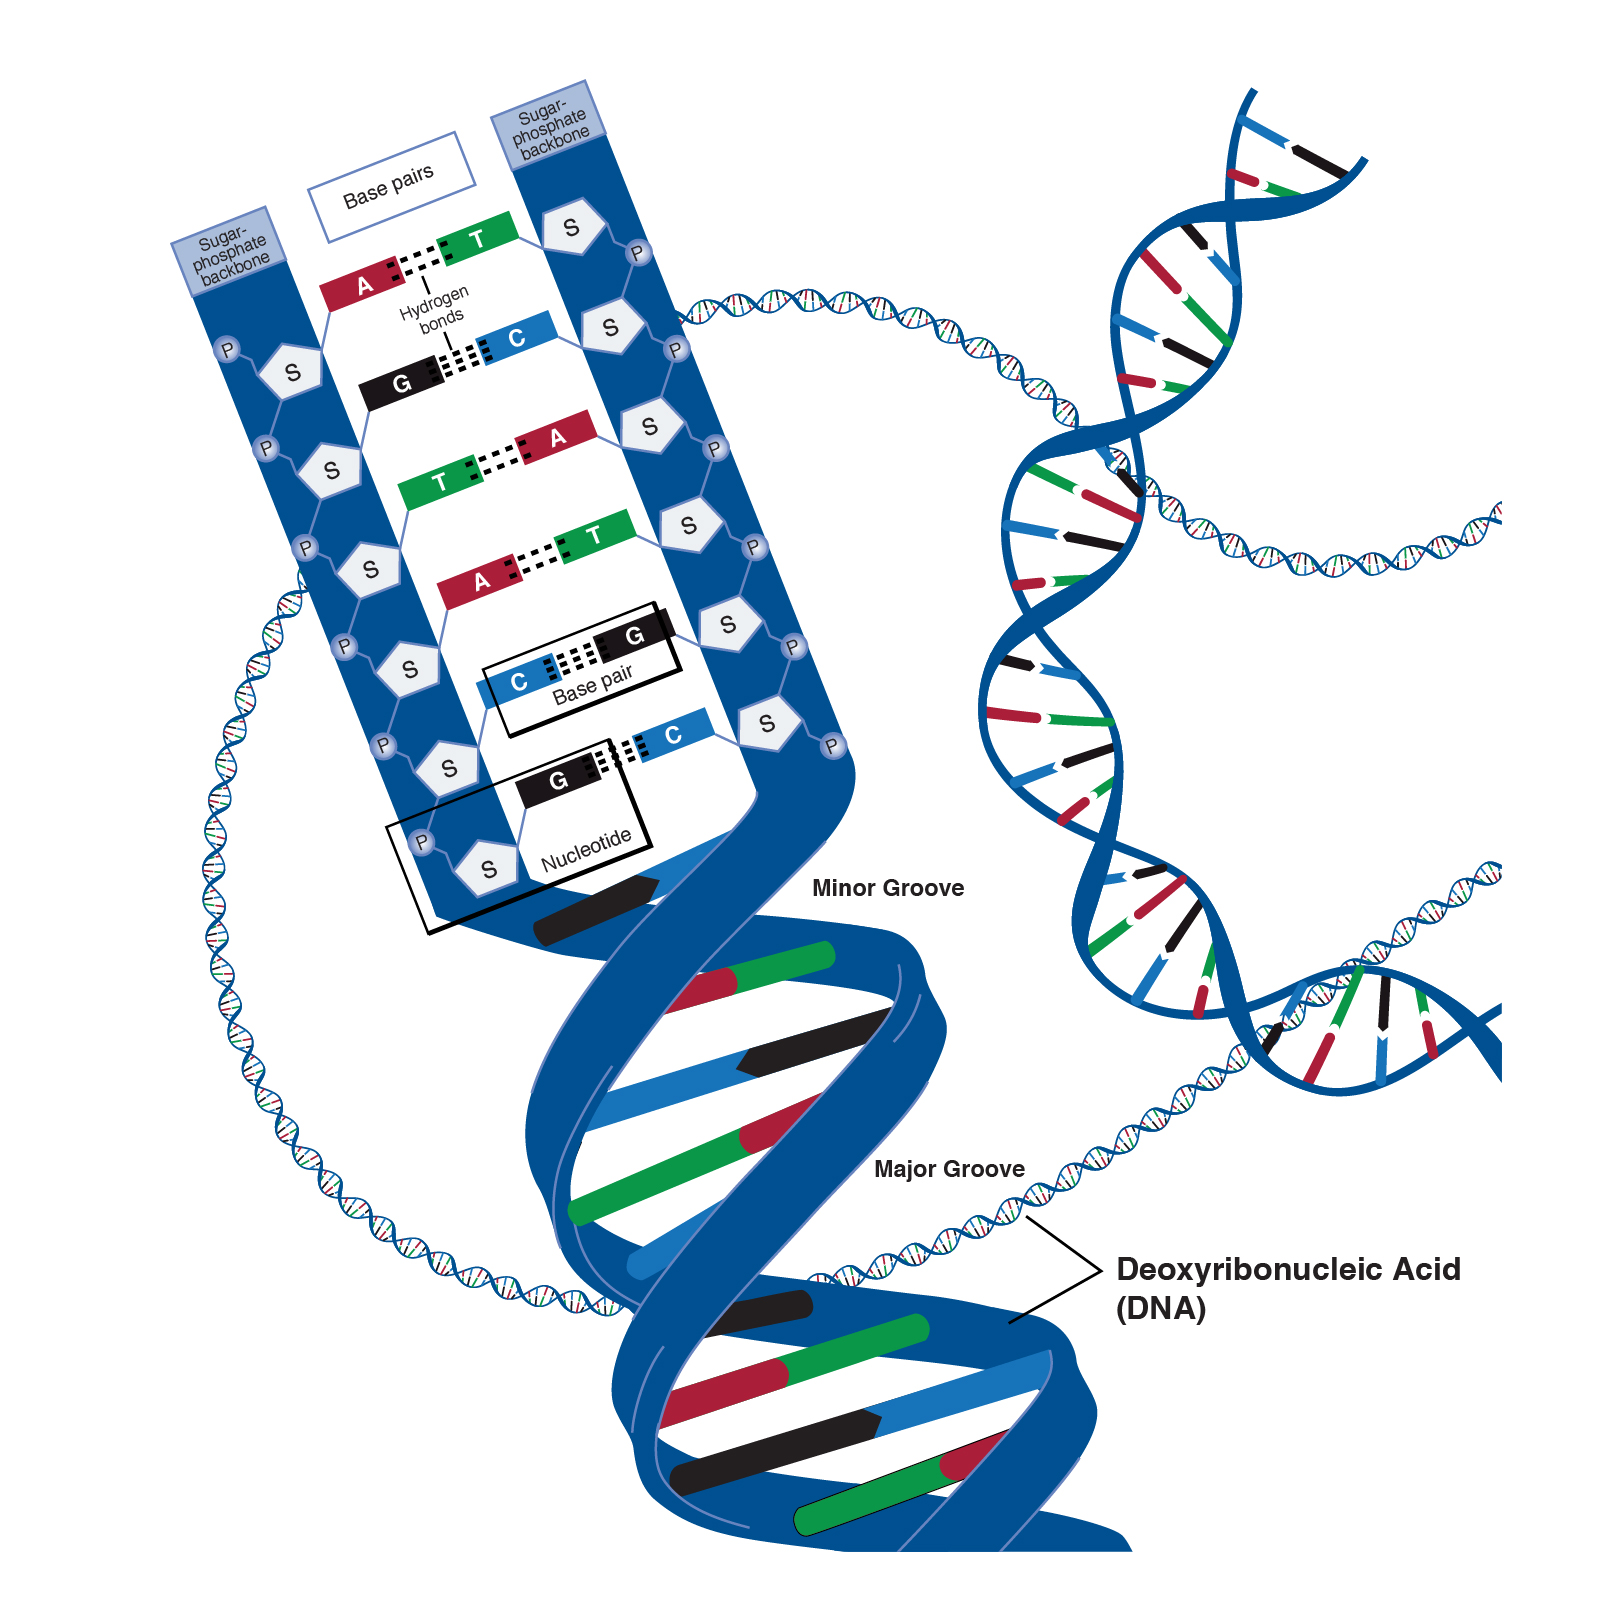
\includegraphics[scale=0.15]{figures/dna_structure.jpg} 
\caption{The structure of the DNA double-stranded helix. (source: \url{https://www.genome.gov/genetics-glossary/Deoxyribonucleic-Acid}) \todo{adapt this figure to also include 3' and 5'}}
\end{figure}

\subsection{A short history of DNA sequencing}

The first DNA sequencing techniques were developed in the second half of the 1970's by Fredrick Sanger \cite{Sanger1977} on the one hand and by Maxam and Gilbert \cite{Maxam1977} on the other hand. Both these methods rely on obtaining pieces of the DNA sequence of all possible lengths while knowing which base occurs at the end of the sequence. By running these sequences through a gel that allows the shorter DNA fragments to move faster, the sequences are ordered by length and the full sequence can be inferred by reading through the gel. Sanger's method, now simply known as \emph{Sanger sequencing} became the most popular of the first generation sequencing techniques. In later years this technique wat further improved and automated such that it could be used to sequence the first human genome in the \emph{Human Genome Project} \cite{Venter2001}.

In the begining of the the 21st century, new sequencing methods were developed collectively known as \emph{\gls{ngs}} or Massively-Parallel Sequencing methods. These techniques can perform a large number of sequencing reactions in parallel. This, in turn, led to a large decrease in the cost and time needed to sequence the genome of an organism. While the precise physics and chemistry behind the processes differs between platforms, a typical NGS experiment has the following steps: First, sequencing libraries are created by fragmenting the DNA. Secondly, these libraries have to be amplified to get a signal identifying a nucleotide in the fragment that is strong enough to be detected by sequencing. Several NGS sequencing techniques exist and were commercialised by different competitors such as pyrosequencing by Roche 454 \cite{Margulies2005}, sequencing by synthesis by Solexa/Illumina \cite{Turcatti2008}, sequencing by ligation by AB SOLiD \cite{Shendure2005} and ion semiconductor sequencing by Ion Torrent \cite{Rothberg2011}. However, these days the biggest player in the NGS market is Illumina, with around $90\%$ of all DNA data being produced by Illumina \cite{Illumina2016}.

Recently, a third generation of sequencing technologies has arisen. These technologies separate themselves from NGS technologies by their capability of sequencing single molecules and obviating the need for amplification. These technologies are therefore often refered to as \gls{sms} technologies. The big players in the current SMS-market are Pacific Biosciences \cite{Eid2009} and Oxford Nanopore \cite{Clarke2009}.

\subsection{The typical output of a sequencing experiment}

There is, to today, no method to sequence a complete genome sequence at once. Instead only parts of the sequence are determined at a time. We refer to these parital DNA sequences as \emph{reads}. The length of a read, i.e.\ the number of sequenced nucleotides it contains, is often given in \emph{\gls{bp}}, because of the double-strandedness of DNA. By ensuring the different reads overlap, the full genome can then be inferred or \emph{assembled}. A task that is often compared to trying to solve a jigsaw puzzle of over a bilion pieces. In this context another important parameter of a sequencing experiment is the \emph{sequencing coverage} or \emph{coverage depth}, which is the number of reads that on average overlap with a nucleotide in the original sequence. Typically, some regions are harder to sequence than other and the actual coverage observed at different parts of the DNA sequence can differ significantly from this average coverage. Finally, errors might occur both during the preprocessing of the DNA (e.g.\ library construction and amplification) and during the actual sequencing itself. This can cause several artefacts in the data such as \emph{substitutions} (e.g.\ a nucleotide C in the DNA sequence might occur as G in the read), \emph{deletions} (part of the DNA sequence is missing in the read) or \emph{insertions} (the read contains nucleotides that are not present in the DNA sequence). Different sequencing techniques will often have different characteristic types of errors, as well as a difference in read length and average accuracy obtained.

\section{Next Generation Sequencing Data}

At the inception of next generation sequencing techniques, many different techniques and companies existed.
Illumina's \gls{sbs} technique had serveral advantages. First, paired-end read data can be produced by sequencing both ends of the fragments. Because the original fragment length is known the distance between the read pairs can be estimated. This occurence of the reads in pairs with known distance between them has proven a valuable asset in downstream analyses of the sequencing data. Second, by adding barcodes to the adapters that are attached during library preparation, it is possible to simultaneously sequence multiple sample libraries in one machine run. This increased the throughput significantly.
Nowadays, some platforms such as Roche/454 and AB SOLiD are no longer being developed and NGS data most often implies sequencing data produced by Illumina machines.
% and downstream applications of the data can thus benefit by taking into account the biases and errors specific to Illumina data.

\subsection{Generation: Illumina sequencing}

Illumina library preparation is performed by first randomly fragmenting the DNA sample after which adapters are added to each end of the fragments. The fragments are amplified through a process called bridge-amplification: A flow cell is coated with primers that correspond with the adapters that were added to the fragments. The fragments are fixed to the flow cell as well and their free adapter binds to a complementary primer. This way fragments form a bridge that is copied by free nucleotides complementary to the sequence of the bridge fragment. This process is repeated to create clusters of copies of the DNA fragments. Such clusters are needed to make the light signal during the sequencing stage strong enough for accurate detection. The clusters are sequenced with a technique called \gls{sbs}. Sequencing is performed in cycles such that each cycle one new nucleotide in the sequence of each cluster is determined. In one cycle the sequences in the amplified library are used as templates to which a new (complementary) nucleotide that is labeled with a fluorescent dye, is added. Trough excitation with a laser a fluorescent signal is measured from all clusters which allows to identify the bases \cite{Illumina2010}.
After some cycles the fluorescent signal will start to degrade because not all fluorescent dye from previous cycles is washed away properly, causing noise in the observations. Because of this the reads produced by Illumina sequencing are fairly short. Depending on the machine used, reads are between 50 and 300 \gls{bp} in length.

\paragraph{Possible errors and biases in the reads}

Illumina sequencing data has one of the lowest error rates compared to other sequencing technologies (\todo{find number}). However, some errors are still present. The most frequently made errors made by Illumina sequencing are substitutions. Errors can be caused by confounded fluorescent signal detection, for example because two of no fluorescently labeled nucleotides are attached during one cycle, thus sending out a different coloured signal (this phenomenon is often referred to as phasing). Additionally, errors can be introduced before sequencing by errors during PCR amplification \cite{Pfeiffer2018}. 
What is more important, these errors often do not occur at random, but are biased towards certain parts of the DNA-sequence. Errors often occur more frequently near the end of the read and some types of substitutions occur more frequently than others (for example G replaced by T occurs more frequently). Moreover, certain motifs (sequences of 3 nucleotides) tend to precede an error and long sequences of the same nucleotide often insertions or deletions \cite{Schirmer2016}. 
Finally another type of sequencing bias can occur, coverage bias implies that the reads are not uniformly distributed across the original genome. Genomic regions with for example low or high GC-content are known to suffer low coverage \cite{Ross2013}.

To improve the detection of sequencing errors, Illumina provides a quality score for each \emph{base-call}.
The quality score of a base in a read is defined as follows:
If $p$ is the probability of an error in the base calling, then quality score $q$ is given by: \[
	q = -10 \log_{10}(p)
\]
\todo{uitbreiden + stukje over hoe goed quality scores errors aangeven}

\subsection{Storage: FastQ format}

\subsection{Analysis: de Bruijn graphs}

\section{Probabilistic graphical models}

\subsection{Representation}

\subsection{Inference}

% vim: spell spelllang=en  tw=140

% reset all acronyms after the introduction
\glsresetall

	\part{Own work}

\chapter{Accurate determination of node and arc multiplicities in de Bruijn graphs using conditional random fields}\label{ch2}
\setlength{\epigraphrule}{0pt}
\setlength{\epigraphwidth}{0.75\textwidth}
\epigraph{\textit{Got to find another nice quote \\ multiple lines even?}}{Anonymous}
% vim: spell spelllang=en syntax=tex  tw=140

\chapter{Approximate inference in conditional random fields that represent  de Bruijn graphs}\label{ch3}
\setlength{\epigraphrule}{0pt}
\setlength{\epigraphwidth}{0.75\textwidth}
\epigraph{\textit{I have always been more curious than wise}}{Amber - Ship of Magic, Robin Hobb}
% vim: spell spelllang=en syntax=tex  tw=140


In the development of detox \citep{Steyaert2020} we introduced a Conditional Random Field (CRF) model of the multiplicities of nodes and arcs in a de Bruijn graph. In \citep{Steyaert2020} we determined marginal probabilities of the multiplicity of a node or arc in the de Bruijn graph by constructing a CRF for a neighbourhood of nodes and arcs around the node/arc of interest. The Variable Elimination algorithm was then used to sum out all other variables in the CRF until only the marginal for the node/arc of interest remained.
We see an increase in multiplicity determination accuracy as a larger neighbourhood is used. However, the use of exact inference techniques such as Variable Elimination, remains limited to small CRFs because of the large increase in runtime caused by adding more variables and, more importantly, by adding more connections to the model.

For this reason we want to investigate the use of approximate inference techniques to compute marginal multiplicity probabilities. This could allow us to increase the neighbourhood size and allow us to infer the most likely multiplicity for multiple nodes and arcs simultaneously. Potentially, we could be able to perform computations for all nodes and arcs in a de Bruijn graph in a single approximate inference run, given a single CRF model for the whole graph.

\section{Loopy belief propagation (BP)}

The variable elimination algorithm is a dynamic programming view of efficient exact inference in a PGM. However, another view on exact inference called `message passing' or `belief propagation', allows us to extend exact inference methods to related approximate inference methods.

Remember that the joint probability of a CRF can be written as a factorisation:
\begin{equation}
	P(\mathbf{Y}|\mathbf{X}) = \dfrac{1}{Z(\mathbf{X})}\prod_{i=1}^M \varphi_i(\mathbf{D}_i). \label{eq:joint}
\end{equation}

\paragraph{Clique tree or Junction tree:} A junction tree corresponding with the factorised joint probability of \eqref{eq:joint} is an undirected, acyclic graph $T = (V,E)$ with node labels $C_i \subseteq \mathbf{X} \cup \mathbf{Y}, \; \forall v_i \in V$, such that the following properties hold \cite{Aji2000} 
\begin{enumerate}
	\item $\forall \varphi_j(D_j)$ in the product \eqref{eq:joint} $\exists v_k \in V:\; D_j \subseteq C_k$. 
	\item $\forall v_i,v_j \in V$: $C_i \cap C_j \subseteq C_k$ for all nodes $v_k \in V$ that lie on a path in T between $v_i$ and $v_j$.
\end{enumerate} 

\paragraph{Factor Graph:} 
The factorisation in \eqref{eq:joint} can be represented with a bipartite graph. A first type of nodes represents the variables $Y$ and $X$, while a second type represents the factors $\varphi_i$. Edges in the graph represent the presence of a variable in the scope of a factor \cite{Kschischang2001}. This graph representation for a CRF, is slightly more expressive than the original CRF-graph representation: Several factorisations could lead to the same CRF-graph, while each factorisation has a unique factor graph (TODO: goede bron (evt Kschischang2001)).

Inference in a PGM can be viewed as the passing of messages through the factor graph. Whenever the factor graph is a tree, this is equivalent to exact inference. When the factor graph contains cycles it can be transformed into a tree-structured graph on which the message passing algorithm is exact, but this comes at a, possibly very large, computational cost \citep{Yedidia2005}.

Finding the (interior) stationary points of a constrained Bethe free energy problem is equivalent to finding Belief Propagation fixed points such that all beliefs are positive(\citep{Yedidia2005}, proof via Lagrange multipliers). A sufficient condition for beliefs to be positive is that there are no hard constraints i.e. there is no factor $\varphi_i$ such that $\varphi_i(\mathbf{D}_i)$ for an assignment of $\mathbf{D}_i$.

\subsection{On the convergence of BP}
If none of the factors in the CRF contain zero-entries, we can prove that there  will exist at least one fixed point of the Belief Propagation message passing scheme \citep{Yedidia2005}. Unfortunately, this gives us no guarantees whether the message passing algorithme will actually converge, this might only be the case for specific starting conditions. Nor does it guarantee that this fixed point is a good approximation of the true marginals one is trying to infer.




\chapter{Conclusions}\label{ch6}
\setlength{\epigraphrule}{0pt}
\setlength{\epigraphwidth}{0.75\textwidth}
\epigraph{\textit{The true delight is in the finding out rather than in the knowing.}}{Isaac Asimov}


% vim: spell spelllang=en syntax=tex tw=140 


%\afterpage{\null\blankpage}

    \part{Papers}
    \let\oldchaptername\chaptername
    \let\oldthechapter\thechapter

%    \renewcommand\thechapter{\Roman{chapter}} % if you want roman numbering
    \renewcommand{\chaptername}{Paper}

    \chapter{chapter}
    \label[mypaper]{paper1}
    %\includepdf[pages=-]{papers/paper1.pdf}

    % APPENDIX &
    %%%%%%%%%%%%

%\afterpage{\null\blankpage}

\bookmarksetupnext{level=part} % puts the bookmark at the same level as a part
\begin{appendices}
    \input{listpapers}

\end{appendices}


\backmatter

    \bookmarksetupnext{level=part} % puts the bookmark at the same level as a part
    \bibliography{refs}

\end{document}

% vim: spell spelllang=en
